\chapter*{Melléklet}

\noindent Téglalap:
\begin{figure}[h]
\centering
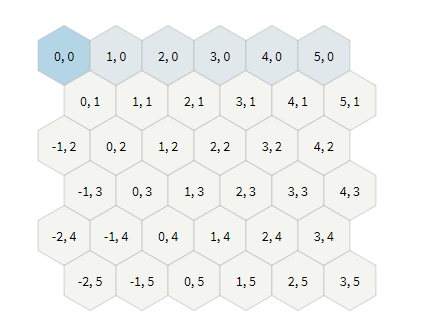
\includegraphics[scale=0.5]{kepek/img_m1.png}
\caption{}
\label{fig:img_m1}
\end{figure}

\begin{figure}[h]
\centering
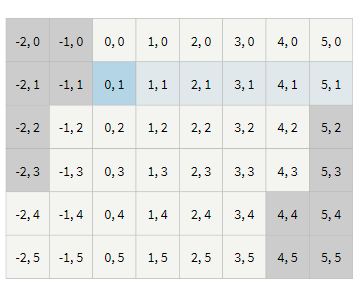
\includegraphics[scale=0.5]{kepek/img_m2.png}
\caption{}
\label{fig:img_m2}
\end{figure}

\noindent Háromszög:
\begin{figure}[h]
\centering
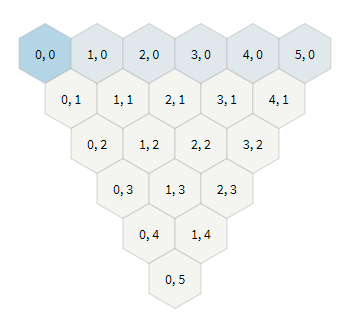
\includegraphics[scale=0.5]{kepek/img_m3.png}
\caption{}
\label{fig:img_m3}
\end{figure}

\begin{figure}[h]
\centering
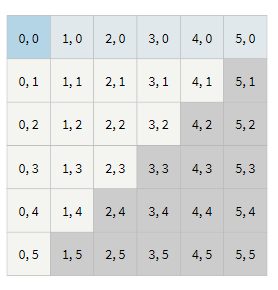
\includegraphics[scale=0.5]{kepek/img_m4.png}
\caption{}
\label{fig:img_m4}
\end{figure}

\noindent Hatszög:
\begin{figure}[h]
\centering
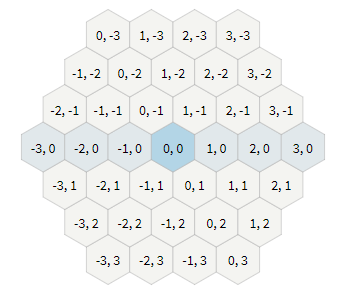
\includegraphics[scale=0.5]{kepek/img_m5.png}
\caption{}
\label{fig:img_m5}
\end{figure}

\begin{figure}[h]
\centering
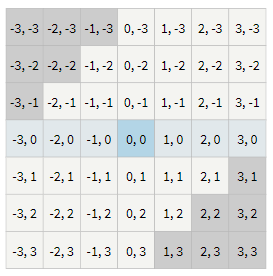
\includegraphics[scale=0.5]{kepek/img_m6.png}
\caption{}
\label{fig:img_m6}
\end{figure}

\noindent Rombusz:
\begin{figure}[h]
\centering
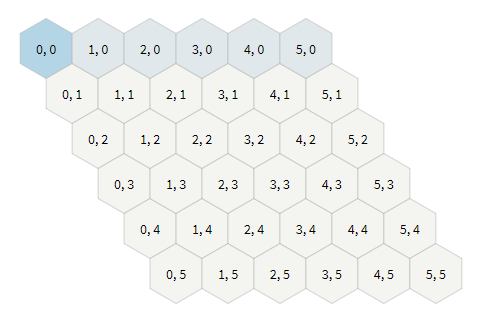
\includegraphics[scale=0.5]{kepek/img_m7.png}
\caption{}
\label{fig:img_m7}
\end{figure}

\begin{figure}[h]
\centering
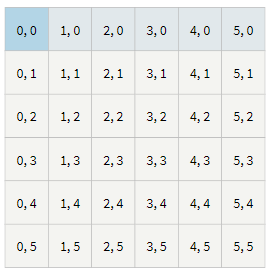
\includegraphics[scale=0.5]{kepek/img_m8.png}
\caption{}
\label{fig:img_m8}
\end{figure}